\section{Vision general del sistema}

Este diagrama respresenta la interacion entre los diferentes elementos de hardware 
y software en una experiencia planificada.

\begin{figure}[!htb].
    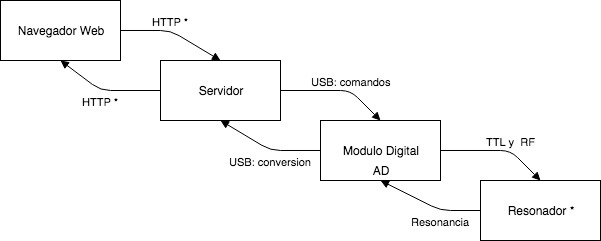
\includegraphics[width=\linewidth]{../figures/d5.jpg}
    \caption{Vision General del sistema}
    \label{fig:d5}
\end{figure}

\subsection{Navegador web}
El navegador web es la plataforma donde se provee al usuario final la interfaz con el sistema.

\subsection{Servidor}
El servidor provee servicios REST solicitados por la interfaz grafica durante la vida
de la sesion del usuario. Estos servicios hacen llamadas al controlador del Modulo
Digital via usb.

\subsection{Modulo Digital}
El modulo digital procesa los mensajes del controlador via usb y ejecuta 
el microcodigo del mismo para la configuracion y ejecucion de las secuencias de pulsos.

\subsection{Resonador}
El resonador recibe los pulsos provenientes del Modulo Digital generando una señal de resonancia
enviada al Modulo Digital para su conversion digital.

\newpage